\documentclass[tikz,border=10pt]{standalone}
% Shared style for all project diagrams
\usepackage{amsmath,amssymb}
\usetikzlibrary{positioning,arrows.meta,calc,fit,decorations.pathreplacing}
\renewcommand{\familydefault}{\sfdefault}
\definecolor{accent}{RGB}{42,120,214}
\definecolor{lblue}{RGB}{234,242,252}
\definecolor{card}{RGB}{247,247,245}
\definecolor{ink}{RGB}{17,17,17}
\definecolor{gray52}{RGB}{82,81,78}
\definecolor{dblue}{RGB}{13,54,107}
\tikzset{
  box/.style={draw=accent, thick, rounded corners=3pt, fill=lblue, align=center,
              minimum height=1.05cm, inner sep=6pt, text=ink},
  plain/.style={draw=gray52!60, thick, rounded corners=3pt, fill=card, align=center,
              minimum height=1.05cm, inner sep=6pt, text=ink},
  ghost/.style={align=center, text=gray52, font=\footnotesize},
  arr/.style={-{Stealth[length=2.6mm]}, very thick, draw=accent},
  garr/.style={-{Stealth[length=2.6mm]}, thick, draw=gray52},
  lbl/.style={font=\footnotesize, text=gray52, align=center},
}

\begin{document}
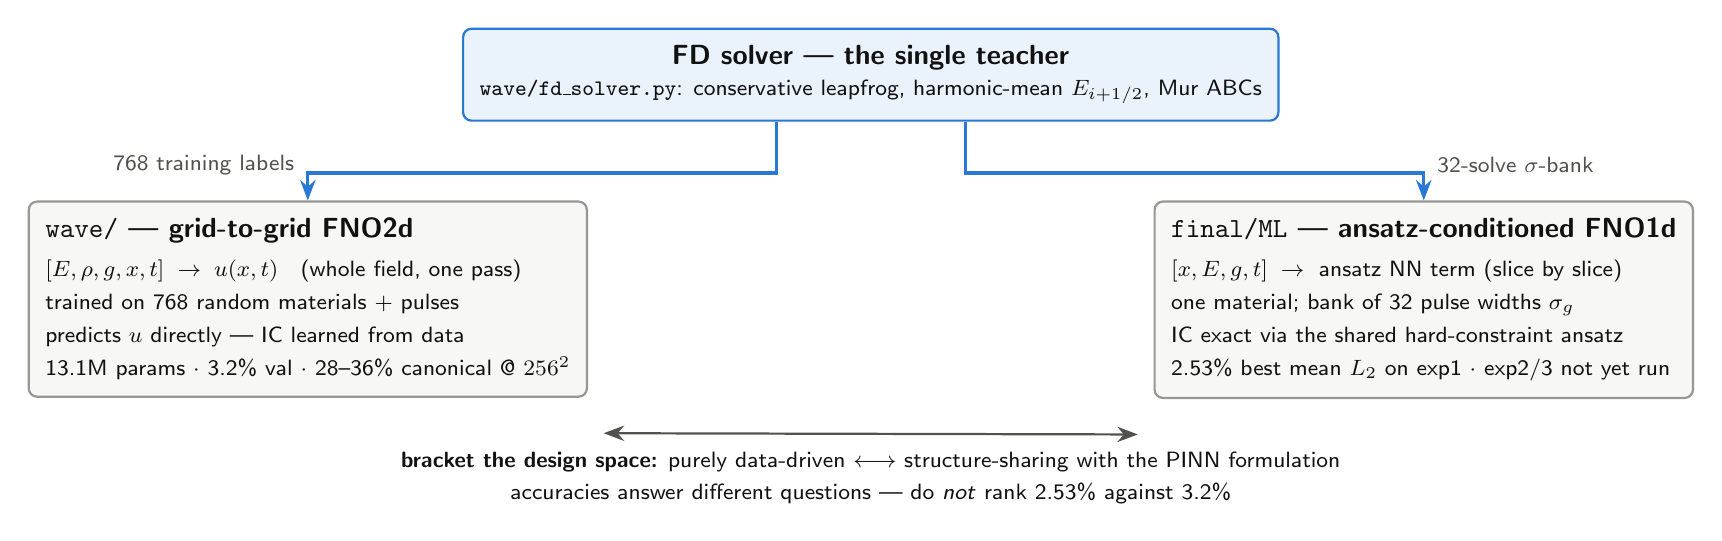
\begin{tikzpicture}[node distance=0.7cm and 1.2cm]
  \node[box, minimum width=5.2cm] (fd)
    {\textbf{FD solver --- the single teacher}\\[-1pt]
     {\footnotesize \texttt{wave/fd\_solver.py}: conservative leapfrog, harmonic-mean $E_{i+1/2}$, Mur ABCs}};

  \node[plain, below left=1.0cm and -1.6cm of fd, minimum width=6.4cm, align=left] (w)
    {\textbf{\texttt{wave/} --- grid-to-grid FNO2d}\\[2pt]
     {\footnotesize $[E,\rho,g,x,t] \;\to\; u(x,t)$ \; (whole field, one pass)}\\
     {\footnotesize trained on 768 random materials + pulses}\\
     {\footnotesize predicts $u$ directly --- IC learned from data}\\
     {\footnotesize 13.1M params $\cdot$ 3.2\% val $\cdot$ 28--36\% canonical @ $256^2$}};

  \node[plain, below right=1.0cm and -1.6cm of fd, minimum width=6.4cm, align=left] (f)
    {\textbf{\texttt{final/ML} --- ansatz-conditioned FNO1d}\\[2pt]
     {\footnotesize $[x,E,g,t] \;\to\; $ ansatz NN term (slice by slice)}\\
     {\footnotesize one material; bank of 32 pulse widths $\sigma_g$}\\
     {\footnotesize IC exact via the shared hard-constraint ansatz}\\
     {\footnotesize 2.53\% best mean $L_2$ on exp1 $\cdot$ exp2/3 not yet run}};

  \draw[arr] (fd.south) ++(-1.2,0) |- ($(w.north)+(0,0.35)$) -- (w.north);
  \draw[arr] (fd.south) ++( 1.2,0) |- ($(f.north)+(0,0.35)$) -- (f.north);
  \node[lbl, left=0.05cm of w.north, yshift=0.45cm] {768 training labels};
  \node[lbl, right=0.05cm of f.north, yshift=0.45cm] {32-solve $\sigma$-bank};

  \draw[garr, {Stealth[length=2.6mm]}-{Stealth[length=2.6mm]}]
    ($(w.south east)+(0.2,-0.45)$) -- ($(f.south west)+(-0.2,-0.45)$)
    node[midway, lbl, below=3pt, text=ink]
    {\textbf{bracket the design space:} purely data-driven $\longleftrightarrow$ structure-sharing with the PINN formulation\\[2pt]
     {\footnotesize accuracies answer different questions --- do \emph{not} rank 2.53\% against 3.2\%}};
\end{tikzpicture}
\end{document}
